\documentclass{article}
\usepackage{gensymb}
\usepackage{textcomp}
\usepackage{amsmath}
\usepackage{hyperref}
\usepackage{bookmark}
\usepackage{float} 
\usepackage{graphicx}
\usepackage{makeidx}
\usepackage[letterpaper, total={7.5in, 10in}]{geometry}

\makeindex
\begin{document}
\title{Circuits (Capacitance and Resistance)}
\author{Elias Xu}
\date{\today}
\maketitle
\setlength{\parindent}{0pt}

\tableofcontents


\section{Introduction}

\begin{figure}[H]
    \centering
    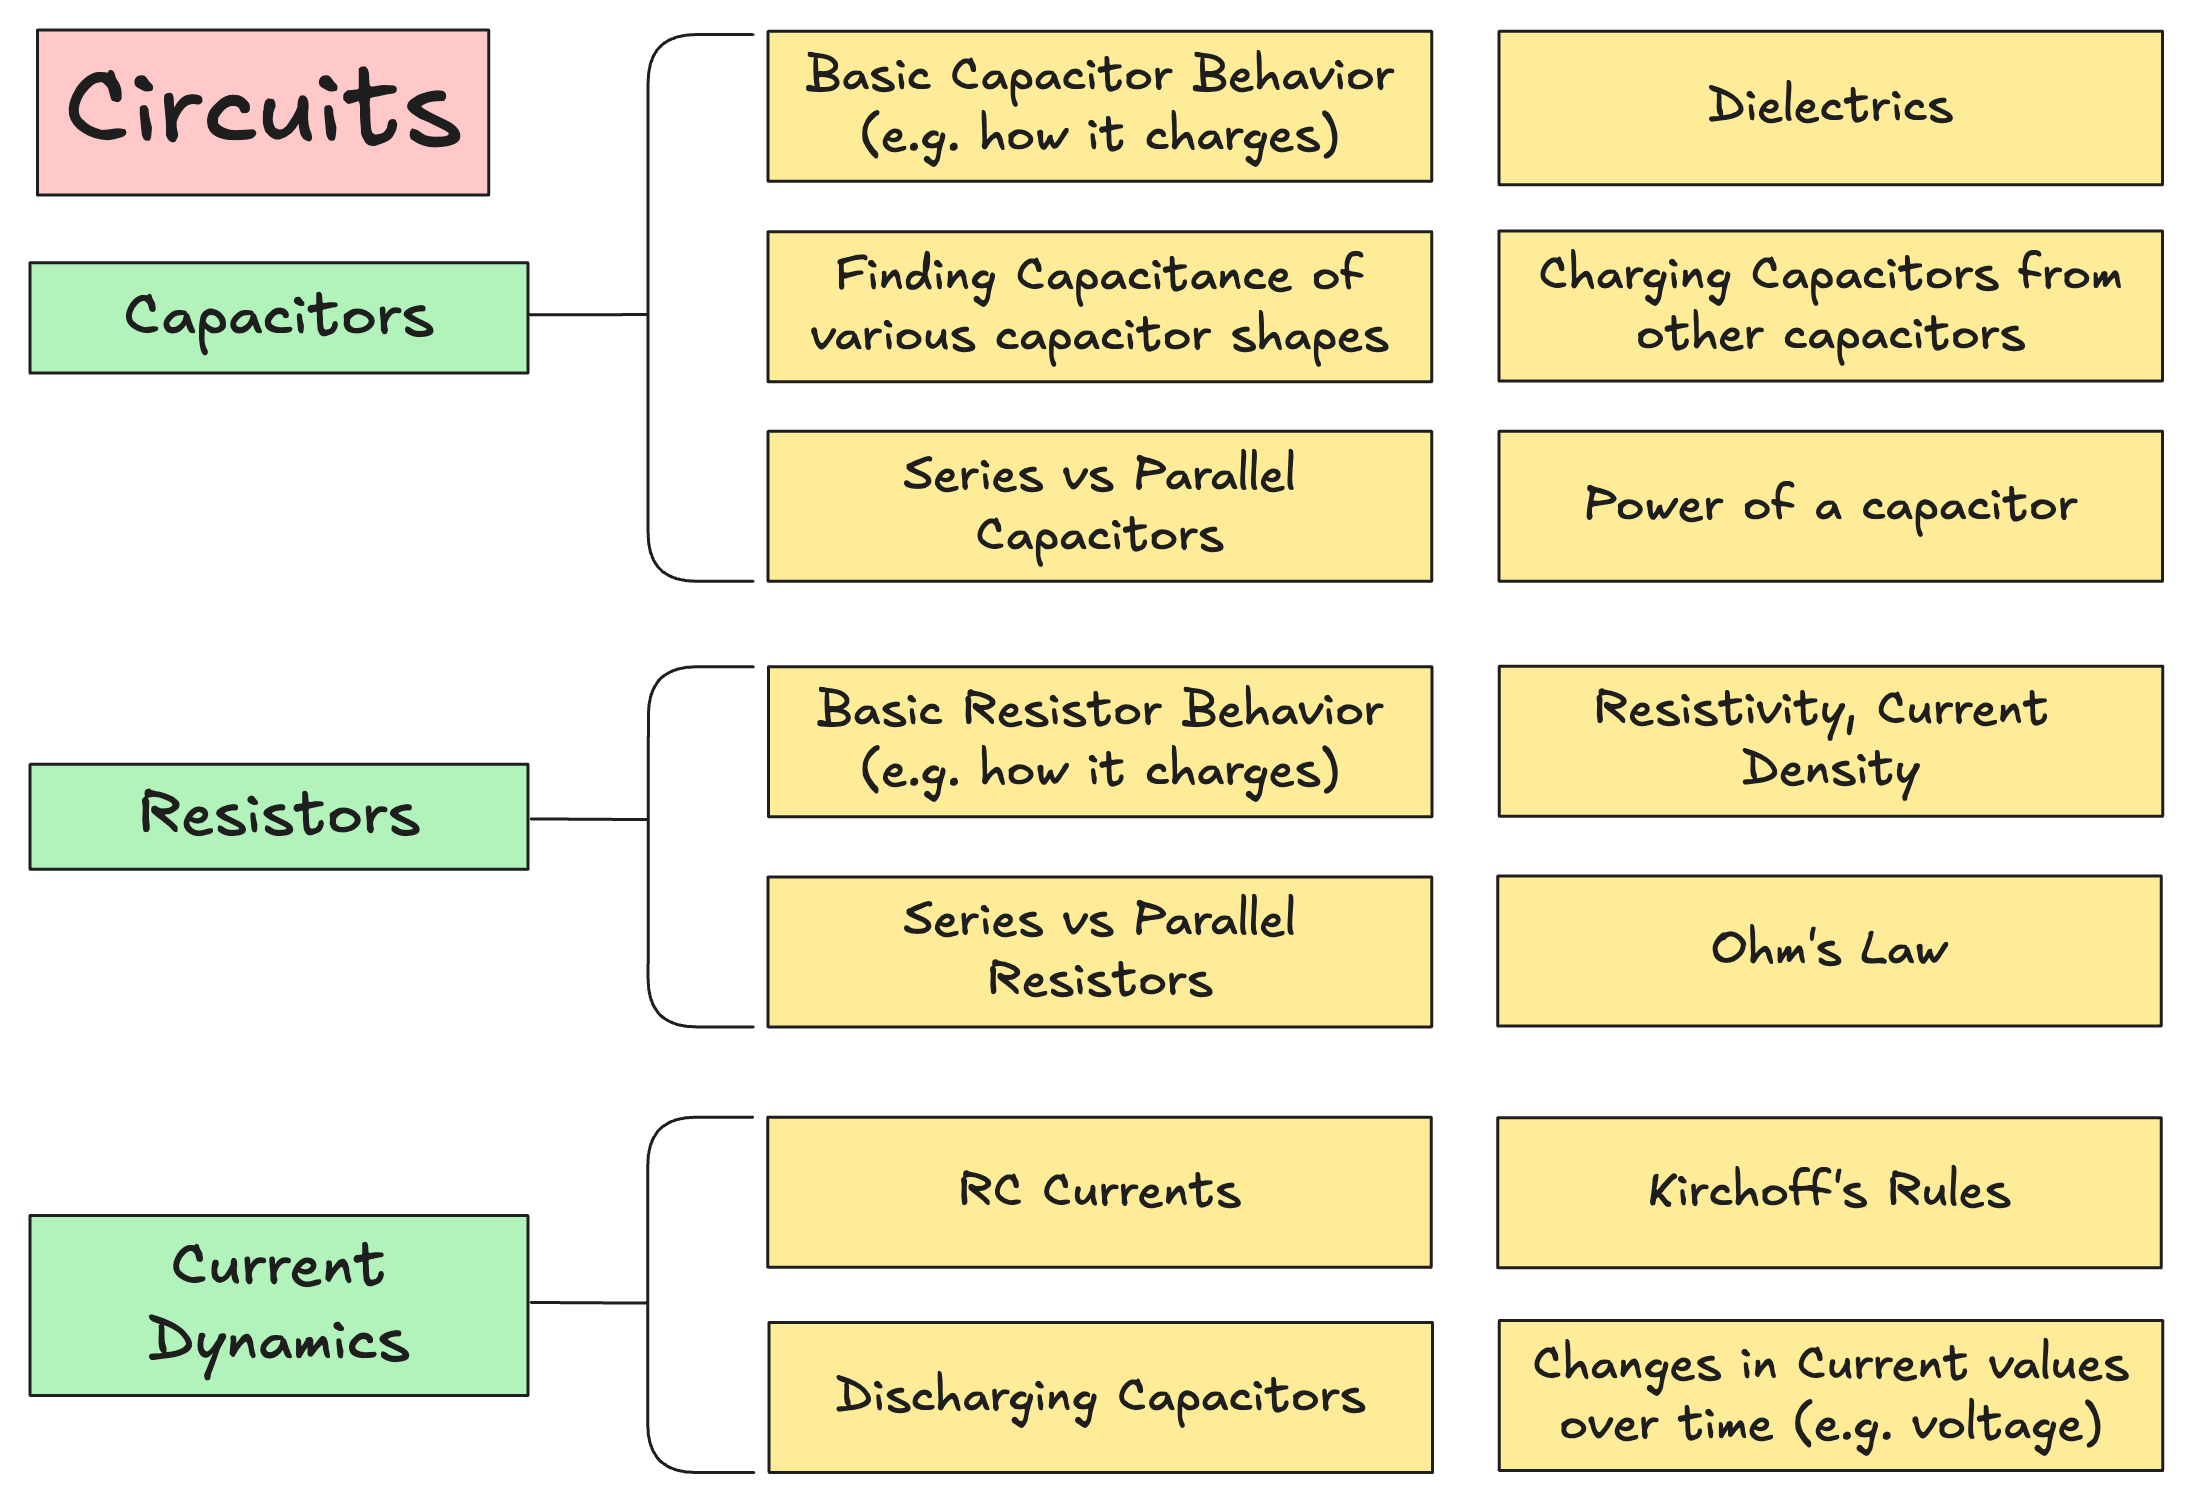
\includegraphics[width=0.8\textwidth]{figures/CicuitryTopicsList.png}
    \caption{Circuitry Topics List}
\end{figure}

\subsection{Basic Intuition for Charge Dynamics}

\begin{itemize}
    \item \textbf{Batteries}: Batteries do NOT supply charges (electrons come from capacitors / wires). Batteries are charge pumps, providing a source of energy.
\end{itemize}

\section{Capacitors}

\subsection{Basic Capacitor Behavior / Intuition}

\begin{itemize}
    \item Capacitors have the ability to store charge over a potential difference
    \item Capacitors are measured in $\text{F}$, or Farads. Unit Analysis: $ \frac{[C]}{[V]} = \frac{[J]}{[C]} = [F]$
    \item Capacitors charge by a batter giving a potential difference between plates, and electrons are then attracted to the different terminals of the battery (bit like gravity)
    \item At $t = 0$, one can treat a capactior as just a regular wire, as as $t \to \infty$, one can treat a capacitor as a broken wire.
\end{itemize}

\subsection{Finding the Capacitance of Capacitor Shapes}

Basic capacitance is calculated by this formula:

$$C = \frac{\text{q}}{\text{V}}$$

Where $q$ is the charge that the conductor has and the $V$ is the potential difference across the capacitor.

Given that capacitance depends on the geometry between the plates, along with the medium between plates, one can calculate the capacitance of a capacitor with an odd geometry by:

\begin{enumerate}
    \item Find the electric field between plates
    \item Find the $\Delta V$ from the field
    \item Apply that to the capacitance equation $C = \frac{q}{V}$
\end{enumerate}

\subsubsection{Finding the Electrical Field between two plates}

With a area of $A$ and a distance between of $d$, with the medium between them air (shown by the $\epsilon_0$)

$$\Phi = EA = \frac{q_{\text{enc}}}{\epsilon_0} = \frac{q}{A \epsilon_0}$$
$$= \frac{\sigma}{\epsilon_0}$$

\subsubsection{Finding voltage from field}

$$\Delta V = - \int \vec{E} \delta \vec{s} = \int_{-\text{plate}}^{+\text{plate}} \vec{E} \delta \vec{s} = E \int \delta s = Ed$$

We removed the negative sign because while the field is going from the positive plate to the negative plate, the direction vector is doing the opposite. We also double the field because of the two plates.

\subsubsection{Solving for capacitance}

$$C = \frac{q}{V} = \frac{q}{\frac{q}{A \epsilon_0}} \times d = \frac{A \epsilon_0}{d}$$

\subsection{Calculating for the Capacitance between Cylindrical Capacitors}

\begin{figure}[H]
    \centering
    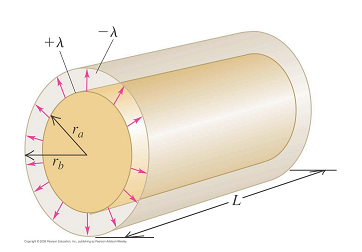
\includegraphics[width=0.3\textwidth]{figures/Cylindrical_Capacitors.png}
    \caption{Examples of a Cylindrical Capacitor}
\end{figure}

\subsubsection{Find Electrical Field between Two of the Cylinders}

$$\Phi = EA = \frac{q_{\text{enc}}}{\epsilon_0}$$
$$A = 2 \pi r L$$
$$E = \frac{q}{2 \pi \epsilon_0 r L}$$

\subsubsection{Find Voltage from Field}

$$\Delta v = - \int \vec{E} \delta \vec{s} = - \int_{b}^{a} \frac{q}{2 \pi r L \epsilon_0} \delta r = \int_{a}^{b} \frac{q}{2 \pi r L \epsilon_0} \delta r = \frac{q}{2 \pi L \epsilon_0} \ln \frac{b}{a}$$

\subsubsection{Solving for the Equation}

$$ C = \frac{q}{v} = \boxed{\frac{2 \pi L \epsilon_0}{\ln \frac{b}{a}}}$$

\subsection{Series and Parallel Capacitors}


Always remember the formula $C = \frac{Q}{V}$

\subsubsection{Capacitors in Parallel}

If a capacitor is in parallel, you can think it as adding up metal plates. Voltages are the same, and charge is proportionate to the capacitance at the capacitor. For an example 3 capacitors in series, the,

$$q_T = V_b \Sigma C $$
$$q_T = q_1 + q_2 + q_3$$
$$V_1 = V_2 = V_3 = V_B$$
$$C_T = C_{\text{eq}} = \frac{q_T}{V_T} = \frac{q_1}{V_1} + \frac{q_2}{V_2}  + \frac{q_3}{V_3}$$
$$C_{\text{eq}} = \Sigma C$$

\textbf{Note}: This is opposite than resistors.

\subsubsection{Capacitors in Series}

If a capacitor is in series, you can think about it as adding up the air gaps. In the end, it's one big capacitor. Thus charge is equal.

$$q_T = q_1 = q_2 = q_3$$
$$V_T = V_1 + V_2 + V_3$$
$$\frac{1}{C_{\text{eq}}} = \frac{V_T}{q_T} = \frac{V_1+V_2+V_3}{q} = \frac{V_1}{q_1} + \frac{V_2}{q_2} + \frac{V_3 }{q_3} = \frac{1}{C_1} + \frac{1}{C_2} = \frac{1}{C_3}$$


\subsection{Dielectrics}

Dielectrics relate to substituting another medium between capacitors other than air. This means that the amount of charge or voltage changes.

\begin{itemize}
    \item \textbf{Case 1: Battery Attached}: Voltage is fixed, which means that only charge can change, and capacitance and charge have a positive linear relationship
    \item \textbf{Case 2: Without Battery}: Charge is fixed, which means that only battery voltage can change, and capacitance and voltage have an inverse relationship
\end{itemize}

\subsubsection{Dieletric intuition}

Normally, when there is a capacitor, the charge difference causes a field to flow uninterrupted through the space between the capacitors. However, when the field flows through a dielectric that has been inserted, the dielectric has a field opposite to the field created by the capacitor.\\
Additionally, if you have a capacitor with different dielectrics split down the middle vertically, you can treat the entire system as two parallel capacitors. If they're split horizontally, then you can treat them as series capacitors.

\subsubsection{Calculating Dielectric}

To account for a new dielectric, we use the Dielectric constant $\kappa$.

$$\kappa = \frac{E_0}{E}$$

Where E is the net electric field ($E_0 - E'$). $\kappa$ always has to be greater than 1, and is dimensionless / without units. We can also gather additional formulas from this earlier formula.

$$E = \frac{q - q'}{A\epsilon_0}$$

$$q' = q(1-\frac{1}{\kappa})$$

\subsection{Charging capacitors from other capacitors}

(e.g. Discharging a charged capacitor into a RC Circuit.)


\begin{figure}[H]
    \centering
    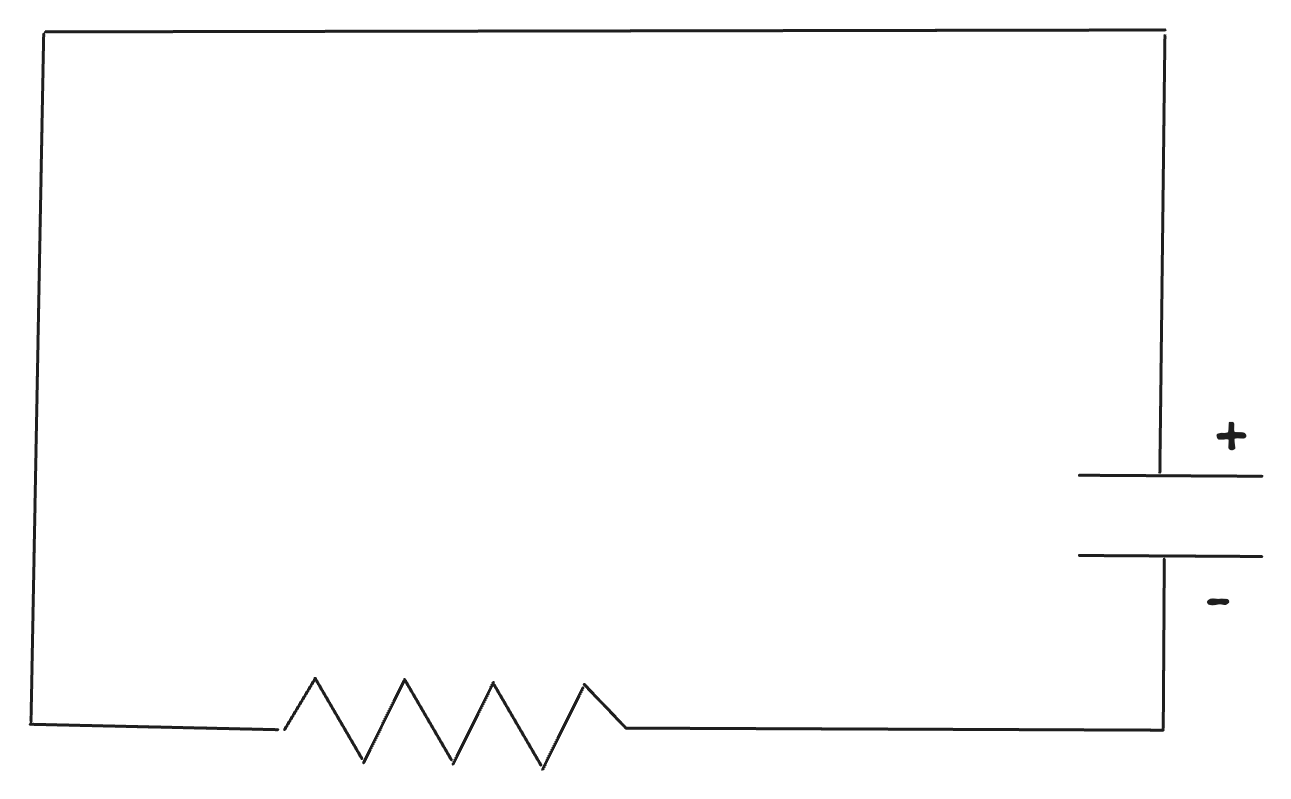
\includegraphics[width=0.3\textwidth]{figures/discharging_capacitor.png}
    \caption{Examples of a Cylindrical Capacitor}
\end{figure}

Given a circuit with a resistor, how does one calculate the charge at a point in time? To solve, calculate it with the current going in the opposite direction (this is to prevent some even more difficult mathematical contortions)

$$\Sigma V = 0 = - \frac{q}{c} - iR = 0$$

$$-\frac{q}{c} - \frac{\delta q}{\delta t} R = 0$$
$$\frac{\delta a}{\delta t} R = - \frac{q}{c}$$
$$\int_{q_0}^{q} \frac{\delta q}{q'} = \int_{0}^{t} \frac{\delta t' }{RC}$$
$$\ln(\frac{q}{q_0}) = - \frac{t}{RC}$$
$$\frac{q}{q_0} = e^{\frac{-t}{RC}}$$
$$q = q_0 e^{-\frac{t}{RC}}$$
$$V_c = \frac{q}{c} = \frac{q_0}{c} e^{-\frac{t}{RC}}$$

You can see the negative sign when you calculate for current, which appears to be negative because of the opposite flow assumption before:

$$i = - \frac{V_0}{Re^{\frac{-t}{RC}}}$$

\subsection{Power/Energy of a capacitors}

One would think that since $q = CV_0$, and since $U = qV$, capacitance is $CV^2$. However, this is not true, since the voltage of a graph changes over time.

$$\Delta U = \int d q \delta U = \int V delta q  = \int \frac{q}{c} \delta q $$
$$ = \frac{q^2}{2c}$$

This can give us a measure about the energy density of an object, $u$,
$$u = \frac{U}{Vol.} = \frac{\frac{CV^2}{2}}{ad} = \frac{\frac{a \epsilon_0 }{d} \times \frac{v^2}{2}}{ad} = \frac{\epsilon_0 V^2}{2 d^2} = \frac{1}{2} \epsilon_0 E^2$$

\section{Resistors}

\subsection{Basic Resistor Behavior / Intuition}

\begin{itemize}
    \item Resistors convert voltage into heat energy (usually heat energy, but also can be light and stuff)
\end{itemize}

\subsection{Series vs Parallel Resistors}

Similar / Different to series / parallel capacitors

\subsubsection{Series Resistors}

(e.g. squeezing the hose at different points).

$$I = I_1 = I_2 = I_3 = ...$$
$$V = V_1 + V_2 + V_3 + ...$$
$$R_{eq} = R_1 + R_2 + R3 + ...$$

Current in all series resistors are equal and since $i = \frac{V}{R}$, voltages add up to battery voltages and resistances all add up to the sum of resistors.

\subsubsection{Parallel Resistors}

(e.g. splitting up the hose into multiple smaller hoses)

$$I = I_1 + I_2 + I_3 + ...$$
$$V = V_1 = V_2 = V_3 = ...$$
$$\frac{1}{V_{eq}} = \frac{1}{R_1} + \frac{1}{R_2} + \frac{1}{R_3} + ...$$

The amount of "water pressure" is the same, but the actual current flowing through is different. 

\subsection{Resistivity, Current Density}

Resistivity is a measure of how "resistant" a circuit, or an object in a circuit is. It's most obvious use is Ohm's Law ($I = \frac{V}{R}$). Resistivity can be defined as:

$$\rho = \frac{E}{J}$$

Where J is the current density, calculated as $\frac{i}{A}$.

Then you can simplify:

$$\rho = \frac{E}{J} = \frac{V / L}{i / A} = \frac{V}{i} \times \frac{A}{L} = R \frac{A}{L}$$

$$R = \frac{\rho L}{A}$$

\subsubsection{Energy Density}

Energy density is literally just the energy divided by the volume.

$$u = \frac{U}{\text{vol}} = \frac{\epsilon_0 V^2}{2 d^2 } = \frac{1}{2} \epsilon E^2$$

\subsubsection{Current Density}

J = $\frac{\delta i}{\delta A} = \int J \delta A$

The speed of electrons in a wire is VERY SLOW, the quantity of electrons give it its power.

\subsection{Resistance}

You can calculate for the resistance of a resistor, given the formula $J = I/A$

$$\rho = \frac{E}{J} = \frac{V / L}{i / A} = \frac{V}{i} \frac{A}{L} = R \frac{A}{L}$$
$$R = \frac{\rho L }{A}$$

\subsection{Electrical Power}

$$i = \frac{\delta q}{\delta t}$$
$$P = \frac{\delta w}{\delta t} = \delta q V = i \delta t V $$
$$P = iV$$

\subsection{Ohm's Law}

Ohm's law relates voltage to current.

$I = \frac{V}{R}$

\section{Current Dynamics}

\subsubsection{Current}

Current is the measure of the flow of <imaginary> positive charges through a wire (which is basically the inverse of electrons, thanks Ben Franklin). Basically, it is the OPPOSITE flow of negatively charge electrons moving through the wire.

Current = i = $\frac{\delta q}{\delta t}$

Units: [i] = $\frac{C}{S}$ = A (Amperes). \\
Current going inside must be the same going outside, e.g. it is conserved.

\subsection{Intuition about Currents}

\begin{itemize}
    \item Again from earlier, capacitors initially act as a wire that as time approaches $\infty$ it then appears as a broken wire (this means that a capacitor doesn't charge all at once, especially if the resistance is large).
\end{itemize}

\subsection{RC Currents (Resistor + Capacitor + Battery)}

$$\Sigma V = V_b + V_r + V_c = \epsilon - iR - \frac{q}{c}$$

[In this case, the voltage of the resistor is negative because it is going with the current].

$$\epsilon - \frac{\delta q}{\delta t} - \frac{q}{c} = 0$$
$$\frac{\delta q}{\delta t} = \frac{\epsilon}{R} - \frac{q}{CR} = \frac{EC - q}{CR}$$
$$\frac{\delta q}{EC - q} = \frac{\delta t}{RC}$$
$$\int_{0}^{q} \frac{\delta q'}{EC - q'} = \int_{0}^{t} \frac{\delta t'}{CR} $$

Adding the primes here because we want to integrate over a range (just differentiating values).

$$-\ln(EC - q')|_{0}^q = \frac{t}{RC}$$
$$\ln(\frac{EC - q}{EC}) = \ln(1-\frac{e}{EC}) = - \frac{t}{RC}$$
$$1 - \frac{q}{EC} = e^{-\frac{t}{RC}}$$
$$q = EC(1-e^{-\frac{t}{RC}})$$

From this equation, you can derive the rest

$$V = \epsilon(1-e^{-\frac{t}{RC}})$$
$$i = \frac{\delta}{\delta t} q = \frac{\epsilon}{R} e^{-\frac{t}{RC}}$$

\subsection{Capacitive Time Constant}

This can give us constants for all capacitors / RC circuits, because R and C is really all that matters. The capacitive time constant is in units of seconds.

$$\tau = RC$$

\subsection{Kirchhoff's Rules}

There are two Kirchhoff's rules, both of which refer to the conservation of something\dots \\
You also get the concept of EMF, electromotive force, from these laws, which is usually provided by either a capacitor or a battery.

\subsubsection{Kirchhoff's Voltage Rule}

\begin{itemize}
    \item All voltages around a loop of a circuit sums together 
    \item For a source of EMF (electromagnetic force, i.e. \emph{voltage}), voltages are positive when  moving from a negative to a positive plate.
    \item The voltage of a resistor are negative when moving in the direction of current.
    \item i.e. conservation of energy
\end{itemize}

In essence, you can sum up the voltages of a circuit either clockwise or counterclockwise, and the should sum to zero (additionally, all objects on the same unsplit wire should have the same current).

\subsubsection{Kirchhoff's Junction Rule}

\begin{itemize}
    \item The sum of all currents entering a junction must be equal to the sum of all currents leaving a junction
    \item i.e. conservation of charge
\end{itemize}

\subsubsection{Loop Rule}

Voltages can be calculated / worked with through the Kirchhoff's voltage rule in a loop, but remember to specify the direction you're calculating with along with the direction of current for the resistors. If you get them wrong, you simply get an inverse, which isn't bad at all.

\subsection{Changes in Circuit Values over Time}

[Remember to draw graphs regarding the formulas, just to gain intuition.]


\end{document}